%%%%%%%%%%%%%%%%%%%%%%%%%%%%%%%%%%%%%%%%%%%
%                                         %
% Title   : m_d.tex                       %
% Subject : Maintenance manual of Scotch  %
%           Data structure explanations   %
% Author  : Francois Pellegrini           %
%                                         %
%%%%%%%%%%%%%%%%%%%%%%%%%%%%%%%%%%%%%%%%%%%

\section{Data structure explanations}
\label{sec-data}

This section explains some of the data structures implemented in
\scotch\ and \ptscotch.

\subsection{\texttt{Dorder}}
\label{sec-data-dorder}

Distributed orderings are data structures used in \ptscotch\ to
represent orderings distributed on a set of processing elements. Like
for the centralized ordering of type \texttt{Order} (see
Section~\ref{sec-data-order}), a distributed ordering consists of an
inverse permutation, which provides the old indices of the reordered
vertices, and a column block decomposition of the reordered matrix, to
help perform more efficient block computations at the solve stage. The
column block decomposition is defined as a tree structure, the nodes
of which, of type \texttt{Dorder\lbt Cblk}, represent column blocks
tree nodes containing consecutive, reordered vertices. A tree node may
have children nodes, which represent the decomposition of a column
block into sub-column blocks, \eg, when a subdomain is decomposed into
two separated subdomains and a separator.

Because its column blocks are distributed across multiple processing
elements, the \texttt{Dorder} data type is much more complex than
the \texttt{Order} data type. Hence, it is important to fully
understand the \texttt{Order} data type before delving into the
meanders of the \texttt{Dorder} data type and its ancillary data
types. The main difference between the two is that, since graphs are
distributed across multiple processing elements, column block
information has to be duplicated on all the processing elements
which contain a piece of a given graph. In order to reconciliate this
information, to provide a centralized block column ordering, all
distributed column block tree node structures are identified by a
\texttt{Dorder\lbt Index} data structure.

The distributed column block tree data structure, created by way of
parallel graph separation algorithms, always ends up in leaves, when
nested dissection no longer succeeds or when the distributed subgraphs
are folded onto single processing elements. As soon as the latter
happens, a purely sequential graph ordering process can take place on
each of them. This leads to the creation of a leaf
\texttt{Dorder\lbt Cblk} node, into which the resulting
locally-computed, centralized column block sub-tree is compacted as an
array of \texttt{Dorder\lbt Node} data structures. From the above, at
the time being, the distributed column block tree structure contains
only either nested dissection nodes, of type
\texttt{DORDER\lbt CBLK\lbt NEDI}, and leaf nodes, of type 
\texttt{DORDER\lbt CBLK\lbt LEAF}. In order to facilitate the
integration of centralized column block sub-trees into a global
distributed column block tree, the values of the type flags are the
same for the \texttt{Dorder} and \texttt{Order} data types.

The fields of the \texttt{Dorder} data structure are the following:
\begin{itemize}
\iteme[\texttt{baseval}]
  Base value for the inverse permutation.
\iteme[\texttt{vnodglbnbr}]
  Overall number of node vertices to order across all processing
  elements. For graph orderings, this number is equal to the number of
  non-halo vertices in the initial graph.
\iteme[\texttt{cblklocnbr}]
  Local number of locally-rooted column blocks. This number is the sum
  of the number of centralized column blocks, of type
  \texttt{Dorder\lbt Node}, held by the current processing element,
  plus the number of distributed column block tree nodes, of type
  \texttt{Dorder\lbt Cblk}, the \texttt{proc\lbt loc\lbt num} index of
  which is equal to the rank of the processing element. This allows
  one to count only once each distributed column block tree node, when
  summing the \texttt{cblk\lbt loc\lbt nbr} fields over all
  processing elements.
\iteme[\texttt{linkdat}]
  Start of the doubly-linked list of distributed column block tree
  nodes, of type \texttt{Dorder\lbt Cblk}, on the given processing
  element. This list is circular, to allow for the insertion of new
  nodes at the end of the list in constant time.
\iteme[\texttt{proccomm}]
  MPI communicator for managing the distributed ordering. It should be
  the same as that of the initial distributed graph to be ordered.
\iteme[\texttt{proclocnum}]
  Rank of the given processing element within the communicator.
\iteme[\texttt{mutelocdat}]
  When multi-threading is activated, allows one to create critical
  sections to update the ordering data in a thread-safe manner.
\end{itemize}

\subsubsection{\texttt{DorderIndex}}
\label{sec-data-dorder-index}

Since the ordering data structure is distributed, pointers cannot be
used to refer to parent or children column block tree node data
structures across processing elements. The \texttt{Dorder\lbt Index}
data type defines an identifier for column block tree nodes. These
identifiers are unique, in the sense that, on each processing element,
no two \texttt{Dorder\lbt Cblk} structures will have the same
identifier. However, several \texttt{Dorder\lbt Cblk} structures may
bear the same \texttt{Dorder\lbt Index} values on different processing
elements, in the case when they are siblings which maintain the local
information about the same distributed column block tree node.

The fields of the \texttt{DorderIndex} data type are the following:
\begin{itemize}
\iteme[\texttt{proclocnum}]
  Smallest rank among the processing elements on which a copy of the
  column block tree node resides.
\iteme[\texttt{cblklocnum}]
  Local number of the column block tree node data structure on the
  processing element of aforementioned rank.
\end{itemize}

\subsubsection{\texttt{DorderLink}}
\label{sec-data-dorder-link}

Since distributed column block tree nodes, of type
\texttt{Dorder\lbt Cblk}, are created on the fly on each processing
element, are in small numbers, and are heavy structures, they are not
stored in a single resizable array, but as individual cells which are
allocated when needed. Consequently, these structures have to be
linked together, for proper management.

The \texttt{DorderLink} data type aims at chaining all
\texttt{Dorder\lbt Cblk} structures in a circular, doubly-linked
list. New nodes are inserted at the end of the list, such that a simple
traversal yields nodes in ascending creation order, which is essential
for locally-rooted nodes when gathering them to create a centralized
ordering. The \texttt{Dorder\lbt Link} structure is the first field of
the \texttt{Dorder\lbt Cblk} structure, so that a simple pointer cast
allows one to retrieve the tree node structure from the current link.

The fields of the \texttt{DorderLink} data structure are the following:
\begin{itemize}
\iteme[\texttt{nextptr}]
  Pointer to the next distributed column block tree node created on
  the given processing element.
\iteme[\texttt{prevptr}]
  Pointer to the previous distributed column block tree node created
  on the given processing element.
\end{itemize}

\subsubsection{\texttt{DorderNode}}
\label{sec-data-dorder-node}

The distributed column block tree data structure ends up in leaves,
when either the parallel nested dissection stops, or when distributed
subgraphs are located on single processing elements. In the first
case, the distributed subgraph is centralized, after which, in both
cases, a centralized ordering strategy is applied to the centralized
subgraph, and a centralized block ordering is computed. This
centralized block ordering is represented as an \texttt{Order}
data structure, containing an inverse permutation and a tree of
\texttt{Order\lbt Cblk} nodes. Since the distributed ordering will
eventually have to be centralized, the local, centralized orderings
will have to be compacted and sent to the root processing
element. In order to anticipate this and to save space, once a
centralized ordering is computed on some processing element, the
resulting column block tree is compacted into a single array of
\texttt{Dorder\lbt Node} cells.

The fields of the \texttt{DorderNode} data type are the following:
\begin{itemize}
\iteme[\texttt{fathnum}]
  Un-based index of the father node of the given node in the node
  array, or $-1$ if the given node is a local root and has to be
  connected to the father of the local leaf of the distributed column
  block tree.
\iteme[\texttt{typeval}]
  Type of centralized column block tree node. The admissible values
  are constants of the kind \texttt{ORDERCBLK*}.
\iteme[\texttt{vnodnbr}]
  Number of node vertices in the column block.
\iteme[\texttt{cblknum}]
  Rank of the tree node among the children of its father, starting
  from zero.
\end{itemize}

Like for the \texttt{Dorder\lbt Cblk} data type, there are no
references from a node to its children, but a reference from each node
to its father, with all information needed to rebuild a global
centralized column block tree when all node information is centralized
on a single processing element.

\subsubsection{\texttt{DorderCblk}}
\label{sec-data-dorder-cblk}

The \texttt{DorderCblk} data type represents distributed column block
tree nodes within distributed orderings. A tree node may be a leaf
node, or have children nodes which describe the decomposition of a
column block into sub-column blocks, \eg, when a graph is decomposed
into two separated subgraphs and a separator.

Since, by nature, every distributed column block tree node concerns a
set of vertices distributed across a set of processing elements, each
of the latter holds a copy of the tree node, the identifier of which,
of type \texttt{Dorder\lbt Index}, contains identical information: the
smallest rank among the involved processing elements within the
communicator used to manage the distributed ordering, and an index
incrementally generated on this processing element. Unlike for the
\texttt{Order} data type, there are no pointers from a tree node to
its child nodes; on the opposite, the \texttt{Dorder\lbt Cblk} node
contains a \texttt{Dorder\lbt Index} referring to its father node. The
only information a tree node will hold about its children is their
number.

The fields of the \texttt{DorderCblk} data type are the following:
\begin{itemize}
\iteme[\texttt{linkdat}]
  Doubly-linked list structure to chain together all
  the \texttt{Dorder\lbt Cblk} structures on a given processing
  element.
\iteme[\texttt{ordelocptr}]
  Pointer to the distributed ordering to which the given distributed
  column block tree node belongs.
\iteme[\texttt{typeval}]
  Type of tree node; at the time being, it is either
  \texttt{DORDER\lbt CBLK\lbt NEDI} for a nested dissection node, or
  \texttt{DORDER\lbt CBLK\lbt LEAF} for a leaf node.
\iteme[\texttt{fathnum}]
  Identifier of the father of the given column block tree node. If the
  given tree node is a root, the value of the father index is
  \texttt{\{~0, -1~\}}.
\iteme[\texttt{cblknum}]
  Identifier of the given column block tree node. The process number
  is the smallest rank among all the processing elements sharing node
  vertices, and the local number is provided incrementally on this
  processing element.
\iteme[\texttt{ordeglbval}]
  Un-based global start index of the node vertices in the distributed
  column block tree node.
\iteme[\texttt{vnodglbnbr}]
  Number of node vertices contained in the distributed column block
  tree node, over all the involved processing elements. If the
  column block has sub-column blocks, the sum of all the
  \texttt{vnodglbnbr} values of the sub-column blocks must be equal to
  the \texttt{vnodglbnbr} of the column block.
\iteme[\texttt{cblkfthnum}]
  Index of the given column block tree node among its siblings,
  starting from zero.
\iteme[\texttt{data}]
  Union field holding the information concerning either the leaf node
  or the nested dissection node. This field has two sub-fields:
  \begin{itemize}
  \iteme[\texttt{leaf}]
    Leaf field, which has the following sub-fields:
    \begin{itemize}
    \iteme[\texttt{ordelocval}]
      Un-based start index in the global inverse permutation array for
      the local vertices.
    \iteme[\texttt{vnodlocnbr}]
      Number of node vertices in the given permutation fragment.
    \iteme[\texttt{periloctab}]
      Pointer to the local, un-based, inverse permutation fragment
      array, of size \texttt{vnod\lbt loc\lbt nbr}. The values of the
      \texttt{peri\lbt loc\lbt tab} array are based according to the
      \texttt{baseval} field of the \texttt{Dorder} data type.
    \iteme[\texttt{nodelocnbr}]
      Number of local column block tree nodes associated with the
      permutation fragment.
    \iteme[\texttt{nodeloctab}]
      Pointer to the local, un-based, array of local column block tree
      nodes, of size \texttt{node\lbt loc\lbt nbr}.
    \iteme[\texttt{cblklocnum}]
      Un-based index, in \texttt{node\lbt loc\lbt tab}, of the root
      local column block tree node.
    \end{itemize}
  \iteme[\texttt{nedi}]
    Nested dissection field. This field has a single sub-field:
    \begin{itemize}
    \iteme[\texttt{cblkglbnbr}]
      Number of sub-column blocks within this column block. For nested
      dissection, this number is either $2$ (two separated parts and
      no separator) or $3$ (two separated parts and a separator).
    \end{itemize}
  \end{itemize}
\end{itemize}

\subsection{\texttt{Graph}}
\label{sec-data-graph}

Graphs are the fundamental underlying data structures of all the
algorithms implemented in \scotch. The \texttt{Graph} structure is the
foundational data structure, from which subclasses will be derived,
according to the specific needs of the \scotch\ modules. It is
sometimes referred to as the \textit{source graph} structure, with
respect to the \textit{target architecture} \texttt{Arch} onto which
source graphs are to be mapped.

The \texttt{Graph} structure, being a foundational data structure,
does not possess any variable fields related to actual computations,
\eg, partition state variables or an execution context. Such fields
will be found in \textit{active} graphs, \eg, \texttt{Bgraph},
\texttt{Kgraph}, \texttt{Vgraph}.

A \texttt{Graph} is described by means of adjacency lists. These data
are stored in arrays and scalars of type \texttt{SCOTCH\_Num}, as
shown in Figures~\ref{fig-lib-graf-one}
and~\ref{fig-lib-graf-two}. The \texttt{Graph} fields have the
following meaning:
\begin{itemize}
\iteme[\texttt{baseval}]
Base value for all array indexing.
\iteme[\texttt{vertnbr}]
Number of vertices in graph.
\iteme[\texttt{edgenbr}]
Number of arcs in graph. Since edges are represented by both of their
ends, the number of edge data in the graph is twice the number of
graph edges.
\iteme[\texttt{verttax}]
Based array of start indices in $\mathtt{edgetax}$ of vertex
adjacency sub-arrays.
\iteme[\texttt{vendtax}]
Based array of after-last indices in $\mathtt{edgetax}$ of vertex
adjacency sub-arrays.
For any vertex $i$, with $\mathtt{baseval} \leq i < (\mathtt{vertnbr}
+ \mathtt{baseval})$, $(\mathtt{vendtax[}i\mathtt{]}
-\mathtt{verttax[}i\mathtt{]})$ is the degree of vertex $i$, and the
indices of the neighbors of $i$ are stored in $\mathtt{edgetax}$ from
$\mathtt{edgetax[\lbt verttax[}i\mathtt{]]}$ to $\mathtt{edgetax[\lbt
vendtax[}i\mathtt{]} - 1\mathtt{]}$, inclusive.

When all vertex adjacency lists are stored in order in
$\mathtt{edgetax}$, it is possible to save memory by not allocating
the physical memory for $\mathtt{vendtax}$. In this case, illustrated
in Figure~\ref{fig-lib-graf-one}, $\mathtt{verttax}$ is of size
$\mathtt{vertnbr} + 1$ and $\mathtt{vendtax}$ points to
$\mathtt{verttax} + 1$. This case is referred to as the ``compact edge
array'' case, such that $\mathtt{verttax}$ is sorted in ascending
order, $\mathtt{verttax[\lbt baseval]} = \mathtt{baseval}$ and
$\mathtt{verttax[\lbt baseval} + \mathtt{vertnbr]} =
(\mathtt{baseval} + \mathtt{edgenbr})$.
\iteme[\texttt{velotax}]
Optional based array, of size $\mathtt{vertnbr}$, holding the integer
load associated with every vertex.
\iteme[\texttt{vnumtax}]
When the current graph is a subgraph of some initial graph, this
based array, of size $\mathtt{vertnbr}$, holds the initial vertex
indices of the subgraph vertices. This array is not defined (\ie,
$\mathtt{vnumtax} = \mathtt{NULL}$) when the graph is the initial
graph.
\iteme[\texttt{edgetax}]
Based array, of a size equal at least to
$\left(\max_{i}(\mathtt{vendtax[}i\mathtt{]}) -
\mathtt{baseval}\right)$, holding the adjacency array of every
vertex.
\iteme[\texttt{edlotax}]
Optional based array, of a size equal at least to
$\left(\max_{i}(\mathtt{vendtax[} i \mathtt{]}) -
\mathtt{baseval}\right)$, holding the integer load associated with
every arc. Matching arcs should always have identical loads.
\end{itemize}

\begin{figure}
\centering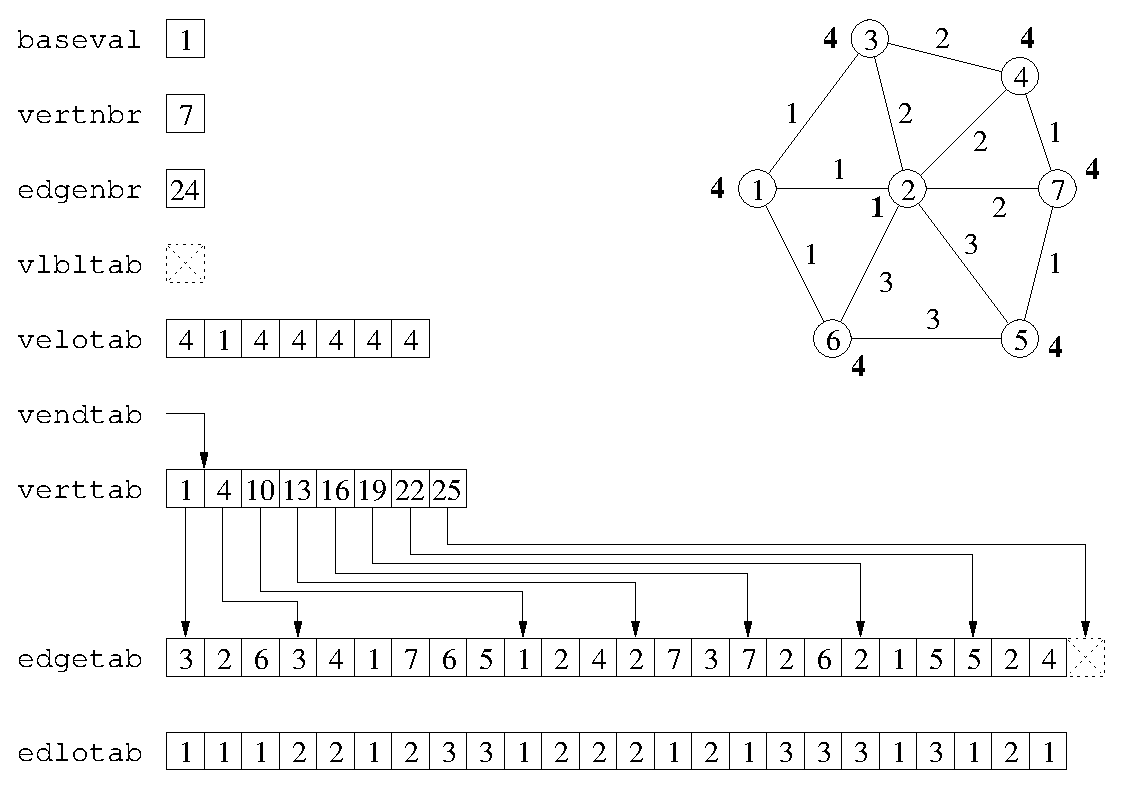
\includegraphics[scale=0.47]{s_f_gr1.eps}
\caption{Sample graph and its description using a compact edge
array. Numbers within vertices are vertex indices, bold numbers
close to vertices are vertex loads, and numbers close to edges are
edge loads. Since the edge array is compact, $\mathtt{verttax}$ is
of size $\mathtt{vertnbr} + 1$ and $\mathtt{vendtax}$ points to
$\mathtt{verttax} + 1$.}
\label{fig-lib-graf-one}
\end{figure}

\begin{figure}
\centering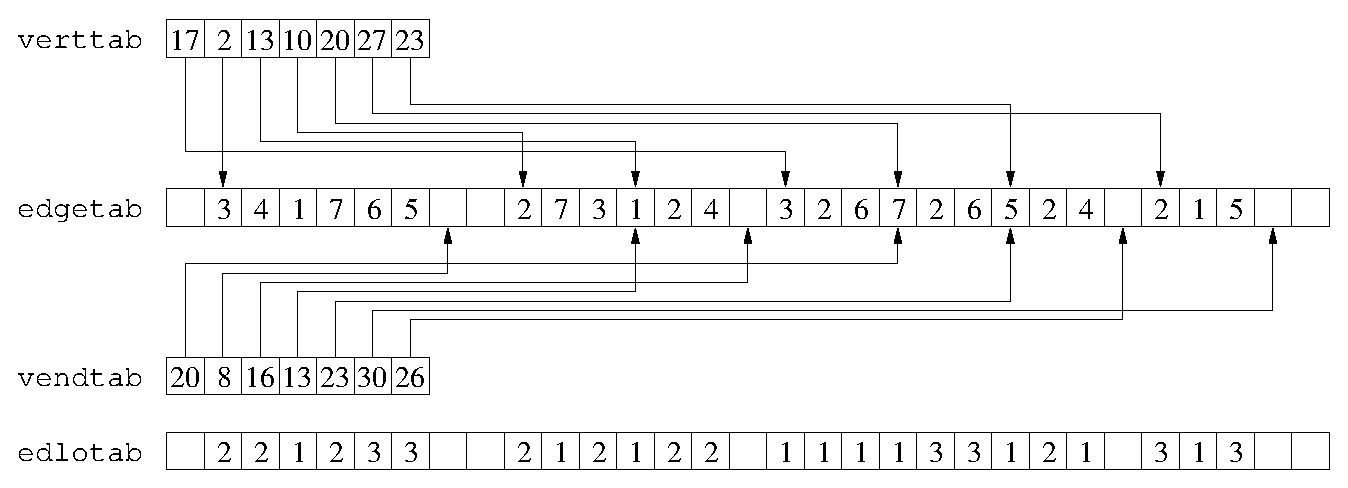
\includegraphics[scale=0.47]{s_f_gr2.eps}
\caption{Adjacency structure of the sample graph of
Figure~\protect\ref{fig-lib-graf-one} with disjoint edge and
edge load arrays. Both $\mathtt{verttax}$ and $\mathtt{vendtax}$ are
of size $\mathtt{vertnbr}$. This allows for the handling of dynamic
graphs, the structure of which can evolve with time.}
\label{fig-lib-graf-two}
\end{figure}

Dynamic graphs can be handled elegantly by using the
$\mathtt{vendtax}$ array. In order to dynamically manage graphs, one
just has to allocate $\mathtt{verttax}$, $\mathtt{vendtax}$ and
$\mathtt{edgetax}$ arrays that are large enough to contain all of the
expected new vertex and edge data. Original vertices are labeled
starting from $\mathtt{baseval}$, leaving free space at the end of the
arrays. To remove some vertex $i$, one just has to replace
$\mathtt{verttax[}i\mathtt{]}$ and
$\mathtt{vendtax[}i\mathtt{]}$ with the values of
$\mathtt{verttax[\lbt vertnbr}\lbt -1\mathtt{]}$ and
$\mathtt{vendtax[\lbt vertnbr}\lbt -1\mathtt{]}$, respectively, and
browse the adjacencies of all neighbors of former vertex
$\mathtt{vertnbr}-1$ such that all $(\mathtt{vertnbr}-1)$ indices are
turned into $i$s. Then, $\mathtt{vertnbr}$ must be decremented.

To add a new vertex, one has to fill $\mathtt{verttax[\lbt vertnbr}
-1\mathtt{]}$ and $\mathtt{vendtax[\lbt vertnbr}\lbt -1\mathtt{]}$
with the starting and end indices of the adjacency sub-array of the
new vertex. Then, the adjacencies of its neighbor vertices must also
be updated to account for it. If free space had been reserved at the
end of each of the neighbors, one just has to increment the
$\mathtt{vendtax[}i\mathtt{]}$ values of every neighbor $i$, and add
the index of the new vertex at the end of the adjacency sub-array. If
the sub-array cannot be extended, then it has to be copied elsewhere
in the edge array, and both $\mathtt{verttax[}i\mathtt{]}$ and
$\mathtt{vendtax[}i\mathtt{]}$ must be updated accordingly. With
simple housekeeping of free areas of the edge array, dynamic arrays
can be updated with as little data movement as possible.

\subsection{\texttt{Hgraph}}
\label{sec-data-hgraph}

The \texttt{Hgraph} structure holds all the information necessary to
represent and perform computations on a \textit{halo} graph. This term
refers to graphs some vertices of which are kept to preserve accurate
topological information, but are usually not subject to actual
computations. These \textit{halo vertices} are collectively referred
to as the \textit{halo} of the graph. Halo graphs are notably used in
sparse matrix reordering, where, in the process of nested dissection,
a graph is cut into three pieces: a vertex separator, and two
separated parts. Each of these parts must preserve the real degree
information attached to all their vertices, including those next to
the separator. If halo graphs were not used, the degrees of these
vertices would appear smaller than what they really are in the whole
graph. Preserving accurate degree information is essential for
algorithms such as the \textit{minimum degree} vertex ordering
method. Some vertex separation algorithms also aim at balancing halo
vertices; in this case, separators will be computed on halos, but this
information will not be preserved once a separator has been computed
on the regular vertices.

Halo graphs exhibit specific structural and topological properties,
illustrated in Figure~\ref{fig-lib-hgraf-one}. In order to distinguish
easily halo vertices from regular vertices and write efficient
algorithms, halo vertices have the highest vertex indices in the
graph. Because the degrees of halo vertices need not be preserved, no
edges connect two halo vertices; the adjacency of halo vertices is
only made of regular vertices. Also, in the adjacency arrays of
regular vertices, all non-halo vertices are placed before halo
vertices. All these properties allow one to easily induce the non-halo
graph from some halo graph, without having to create new adjacency
arrays. An additional vertex index array is present just for this
purpose.

\begin{figure}
\centering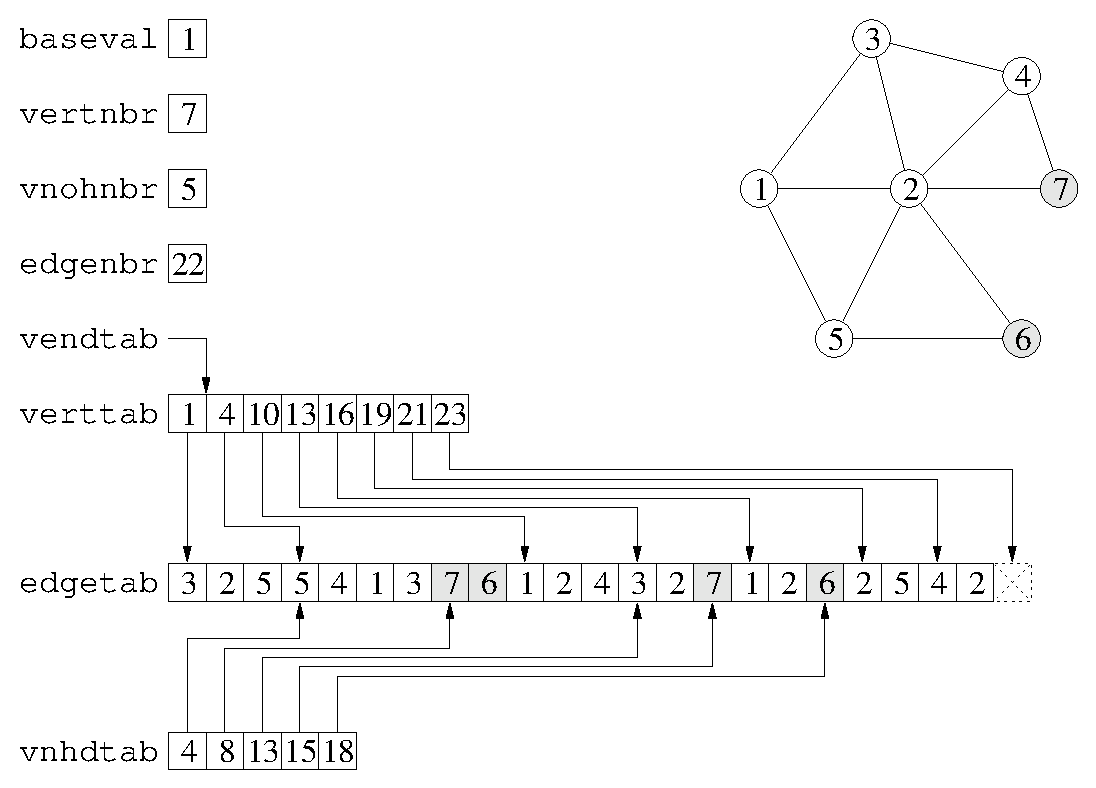
\includegraphics[scale=0.47]{m_f_gr3.eps}
\caption{Sample halo graph and its description using a compact edge
array. Numbers within vertices are vertex indices. Greyed values
are indices of halo vertices. Halo vertices have the highest indices
in the graph, and are placed last in the adjacency sub-arrays of each
non-halo vertex.}
\label{fig-lib-hgraf-one}
\end{figure}

Halo graph fields have the following meaning:
\begin{itemize}
\iteme[\texttt{s}]
Underlying source graph that contains all regular and halo
vertices. This is where to search for fields such as
$\mathtt{baseval}$, $\mathtt{vertnbr}$, $\mathtt{vertnnd}$,
$\mathtt{verttax}$, $\mathtt{vendtax}$, etc.
\iteme[\texttt{vnohnbr}]
Number of non-halo vertices in graph. Hence, $0 \leq \mathtt{vnohnbr}
\leq \mathtt{s.vertnbr}$.
\iteme[\texttt{vnhdtax}]
Array of after-last indices in $\mathtt{s.edgetax}$ of non-halo vertex
adjacency sub-arrays. Since this information only concerns non-halo
vertices, $\mathtt{vnhdtax}$ is of size $\mathtt{vnohnbr}$, not
$\mathtt{vertnbr}$.
For any non-halo vertex $i$, with $\mathtt{baseval} \leq i <
(\mathtt{vnohnbr} + \mathtt{baseval})$, the indices of the non-halo
neighbors of $i$ are stored in $\mathtt{s.edgetax}$ from $\mathtt{s.edgetax}\lbt
\mbox{\texttt{[}}\mathtt{s.verttax}\mbox{\texttt{[}}i\mbox{\texttt{]]}}$
to $\mathtt{s.edgetax}\lbt
\mbox{\texttt{[}}\mathtt{vnhdtax}\mbox{\texttt{[}}i\mbox{\texttt{]}} -
1\mbox{\texttt{]}}$, inclusive, and its halo neighbors are stored from
$\mathtt{s.edgetax}\lbt
\mbox{\texttt{[}}\mathtt{vnhdtax}\mbox{\texttt{[}}i\mbox{\texttt{]]}}$
to $\mathtt{s.edgetax}\lbt
\mbox{\texttt{[}}\mathtt{s.vendtax}\mbox{\texttt{[}}i\mbox{\texttt{]}} -
1\mbox{\texttt{]}}$, inclusive.
\iteme[\texttt{vnlosum}]
Sum of non-halo vertex loads. Hence, $0 \leq \mathtt{vnlosum}
\leq \mathtt{s.velosum}$.
\iteme[\texttt{enohnbr}]
Number of non-halo arcs in graph. Hence, $0 \leq \mathtt{enohnbr}
\leq \mathtt{s.edgenbr}$.
\end{itemize}

\subsection{\texttt{Kgraph}}
\label{sec-data-kgraph}

The \texttt{Kgraph} structure holds all the information necessary to
compute a k-way (re)mapping of some graph onto a target architecture.
Consequently, it contains a \texttt{Graph}, defined as field
\texttt{s}, and a reference to an \texttt{Arch}, through the field
\texttt{m.archptr}, as well as two \texttt{Mapping} structures: one
for the current mapping to compute, and one to store the old mapping
from which to remap. Additional information comprise data to model the
cost of remapping, and data associated with the state and cost of the
current mapping: list of frontier vertices, load of each partition
domain, plus the execution context for multi-threading execution.

The \texttt{Graph} structure is internal to the \texttt{Kgraph}
because every new \texttt{Kgraph} contains a different graph topology
(\eg, a band graph or a coarsened graph). The \texttt{Arch} is
accessed by reference because it is constant data which can be shared
by many \texttt{Kgraph}s. For the sake of consistency, the
\texttt{grafptr} fields of each mapping \texttt{m} and \texttt{r.m}
must point to \texttt{\&s}, while their two \texttt{archptr} fields
must point to the same target architecture. This redundency is the
price to pay for lighter memory management.

\subsubsection{Mappings}

The \texttt{domnorg} field, which must contain a valid domain in the
architecture \texttt{m.archptr}, is the starting point for the k-way
mapping. This domain may be smaller than the full architecture when
parallel partitioning is performed: in this case, each process may
receive a separate subgraph and sub-architecture to work on.

Each of the two mappings has its own specificities. The current
mapping, defined as field \texttt{m}, is never incomplete: all the
cells of its \texttt{m.parttax} array are non-negative values that index
a valid domain in the domain array \texttt{m.domntab}. These domains
are all subdomains of the architecture referenced through field
\texttt{m.archptr}. More restrictively, the domains attached to
non-fixed vertices must be included in \texttt{domnorg}, which may be
smaller.

The current mapping evolves with time, according to the various
algorithms that the user can activate in the strategy string. These
algorithms will create derived \texttt{Kgraph}s (\eg, band graphs or
coarsened graphs), to which mapping methods will be applied, before
the result is ported back to their parent \texttt{Kgraph}. Depending
on the kind of the derived graph, the \texttt{m.parttax} array may be
specific, but the \texttt{m.domntab} array will always be ported back
as is. Consequently, in order to save memory copying, the policy which
is implemented is that the derived \texttt{Kgraph} gets the pointer to
the \texttt{m.domntab} of its parent, while the latter is set to
\texttt{NULL}. The derived graph can therefore reallocate the array
whenever needed, without the risk of an old, invalid, pointer being
kept elsewhere. Then, when the processing of the derived
\texttt{Kgraph} ends, the most recent pointer is copied back to the
\texttt{m.domntab} field of the parent graph, and the
\texttt{m.parttax} array is updated accordingly, after which the
derived \texttt{Kgraph} can be destroyed without freeing the
pointer.

The old mapping, defined as field \texttt{r.m},
may contain incomplete mapping information: some of the cells of its
\texttt{r.m.parttax} array may be equal to \texttt{-1}, to indicate
that no prior mapping information is available (\eg, when the vertex
did not exist in the previous mapping). Since old mappings do not
change, the \texttt{r.m.domntab} field can be shared among all derived
\texttt{Kgraph}s. It is protected from double memory freeing by not
setting the \texttt{MAPPING\lbt FREE\lbt DOMN} flag in field
\texttt{r.m.flagval}.

\subsection{\texttt{Mapping}}
\label{sec-data-mapping}

The \texttt{Mapping} structure defines how individual vertices of a
\texttt{Graph} are mapped individually onto (parts of) an
\texttt{Arch}. A mapping is said \textit{complete} if all source graph
vertices are assigned to terminal target domains, \ie, individual
vertices of the target architecture, or \textit{partial} if at least
one of the source graph vertices is assigned to a target domain that
comprises more than one vertex. In the course of the graph mapping
process, the destination of source vertices are progressively refined,
from an initial target domain that usually describes the whole of the
target architecture, to terminal domains.

Since \texttt{ArchDom}, the data structure that describes target
architecture domains, is big and costly to handle (\eg, to compare if
two \texttt{ArchDom}s are identical), the handling of domains in
mapping is indirect: in the part array \texttt{parttax}, each vertex
is assigned an integer domain index that refers to a domain located in
the domain array \texttt{domntab}. Hence, when two graph vertices have
the same index in \texttt{parttax}, they belong to the same domain and
induce no communication cost. However, the opposite is false: two
vertices may have a different index in \texttt{parttax} and yet belong
to the same target domain. This is for instance the case when one of
the vertices is a fixed vertex that has been set to a specific
terminal domain at initialization time, and one of its neighbors is
successively mapped to smaller and smaller subdomains that eventually
amount to the same terminal domain.

In the case of a remapping, the mapping information regarding the
former placement of the vertices may be incomplete, \eg, because the
vertex did not exist before. Such a mapping is said to be
\textit{incomplete}. It is characterized by the fact that some cells
of the \texttt{parttax} array are equal to \texttt{-1}, to indicate an
unknown terminal domain number. To allow for this, the mapping must
have the \texttt{MAPPING\lbt INCOMPLETE} flag set. Incomplete mappings
are only valid when holding remapping information; new mappings being
computed must have all their \texttt{parttax} cells set with
non-negative values that point to valid domains in the
\texttt{domntab} array. New mappings can therefore only be partial or
complete.

When a mapping is initialized, all \texttt{parttax} values for
non-fixed vertices are set to index~$0$, and \texttt{domntab[0]} is
set to the root domain for the mapping. In the general case for
centralized mapping, the initial domain is equal to
\texttt{archDomFrst(archptr)}. However, when a centralized mapping
process is launched as a part of a distributed mapping process, the
initial domain may be a subset of the whole target architecture.

There is no obligation for the \texttt{domntab} array to contain only
one instance of some target domain. On the contrary, as described
above, the same domain may appear at least twice: once for fixed
vertices, and once for non-fixed vertices on which mapping algorithms
are applied. However, for efficiency reasons (\eg, avoiding to compute
vertex distances that are equal to zero), it is preferable that
duplicate domains are avoided in the \texttt{domntab} array. This is
the case by nature with recursive bipartitioning, as the domains
associated with branches of the biparitioning tree are all distinct.

Making the distinction between fixed and non-fixed vertices, which is
relevant to mapping algorithms, is not in the scope of the
\texttt{Mapping} data structure, which only represents a global
state. This is why no data related to fixed vertices is explicitly
present in the mapping itself (it may be found, \eg, in the
\texttt{Kgraph} data structure).
However, for handling fixed vertices in an efficient way, the
semantics of the \texttt{Mapping} data structure is that all domains
that are associated with fixed vertices must be placed first in the
\texttt{domntab} array. The purpose of this separation is because,
when the imbalance of a mapping is computed, the loads of non-fixed
vertices that belong to some (partial) domain and of fixed vertices
that belong to domains that are subdomains of this domain have to be
aggregated. This aggregation procedure is made easier if both types of
domains are kept separate. For efficiency reasons, fixed domains
should appear only once in the fixed part of \texttt{domntab}.
\\

The \texttt{Mapping} structure is mainly used within the
\texttt{Kgraph} structure, which contains two instances of it: one for
the current mapping to be computed, and one for the old mapping, in
the case of remapping. The building of a \texttt{Kgraph} from another
one (\eg, when creating a band graph or a coarsened graph) may lead to
situations in which some \texttt{Mapping} arrays may be re-used, and
thus should not be freed when the derived \texttt{Mapping} is
freed. This is why the \texttt{Mapping} structure contains flags to
record whether its arrays should be freed or not. These flags are the
following:
\begin{itemize}
\iteme[\texttt{MAPPINGFREEDOMN}]
  Set if the domain array has to be freed when the mapping is freed. A
  common case for sharing the domain array is when a coarser
  \texttt{Kgraph} is computed: the domain array of the coarse old
  mapping can re-use that of the fine old mapping.
\iteme[\texttt{MAPPINGFREEPART}]
  Set if the part array has to be freed when the mapping is freed. A
  common case for sharing the part array is when the user part array
  is kept as the part array for the initial \texttt{Kgraph} current
  mapping structure.
\end{itemize}

The main fields of the \texttt{Mapping} data structure are the following:
\begin{itemize}
\iteme[\texttt{flagval}]
  Set of flags indicating whether the \texttt{parttax} and
  \texttt{domntab} have to be freed on exit.
\iteme[\texttt{grafptr}]
  Pointer to the \texttt{Graph} associated with the mapping, that
  gives access to the base value \texttt{grafptr->\lbt baseval} and
  the number of source vertices \texttt{grafptr->\lbt vertnbr}.
\iteme[\texttt{archptr}]
  Pointer to the \texttt{Arch} associated with the mapping, that is
  necessary to perform all distance computations on the mapping.
\iteme[\texttt{parttax}]
  Based array of \texttt{Anum}s, of size \texttt{grafptr->\lbt
  vertnbr}, that provides the index of the target domains onto which
  all graph vertices are currently mapped. Indices are un-based.
\iteme[\texttt{domntab}]
  Un-based array of \texttt{ArchDom}s, of size \texttt{domnmax}, that
  stores the target domains to which source graph vertices are
  indirectly associated through the \texttt{parttax} array.
\iteme[\texttt{domnnbr}]
  Number of target domain slots currently used in
  \texttt{domntab}. After a mapping is initialized, $1 \leq
  \mbox{\texttt{domnnbr}} < \mbox{\texttt{domnmax}}$, because source
  graph vertices must be associated to some domain, hence
  \texttt{domntab} should at least contain one domain.
\iteme[\texttt{domnnbr}]
  Number of target domain slots currently used in
  \texttt{domntab}.
\iteme[\texttt{domnmax}]
  Size of the \texttt{domntab} array.
\iteme[\texttt{mutedat}]
  When multi-threading is activated, allows to create critical
  sections to update the mapping data in a thread-safe manner.
\end{itemize}

\subsection{\texttt{Order}}
\label{sec-data-order}

Orderings are data structures used in \scotch\ to represent
fill-minimizing block orderings of adjacency matrices represented as
graphs. A block ordering, contained in the \texttt{Order} data
structure, is defined by an inverse permutation, which provides the
old indices of the reordered vertices, and a column block
decomposition of the reordered matrix, to help performing more
efficient block computations at the solving stage.

Inverse permutations are used, instead of direct permutations, because
their processing is more local: when ordering some subgraph, the only
ordering information to provide is the un-based start index, usually
called \texttt{ordenum}, in the inverse permutation vector, usually
called \texttt{peritab}, while the \texttt{vnumtax} array of the
\texttt{Graph} structure holds the values of the vertex indices to
write in the sub-array of \texttt{peritab} starting at index
\texttt{ordenum}, of a size equal to the number of concerned vertices
in the \texttt{Graph}. Once an ordering is computed, it is
straightforward to compute the direct permutation \texttt{permtab}
from the inverse permutation \texttt{peritab}, in case it is needed.

The column block decomposition is defined as a tree structure, whose
nodes, of type \texttt{Order\lbt Cblk}, represent column blocks
containing consecutive, reordered vertices. A tree node may have
ordered children nodes, which represent the decomposition of a column
block into sub-column blocks, \eg, when a subdomain is decomposed into
two separated subdomains and a separator.

The main fields of the \texttt{Order} data structure are the
following:
\begin{itemize}
\iteme[\texttt{flagval}]
Flag that indicates whether the \texttt{peritab} inverse permutation
array has to be freed on exit.
\iteme[\texttt{baseval}]
Base value for inverse permutation values.
\iteme[\texttt{vnodnbr}]
Number of vertex nodes in the ordering. When the associated graph
structure is a \texttt{Graph}, this number is equal to its
\texttt{vertnbr} field; when it is a \texttt{Mesh}, it is equal to
its \texttt{vnodnbr} field.
\iteme[\texttt{treenbr}]
Number of tree nodes in the ordering. This number is equal to $1$ when
only the root tree node is present, and is incremented each time a new
tree node is added to the tree structure.
\iteme[\texttt{cblknbr}]
Number of column blocks in the ordering. This number is equal to $1$
when only the root tree node is present. When some column block
is decomposed into $c$ sub-column blocks, it is increased by $(c-1)$,
since this represents the number of additional column blocks in the
structure.
\iteme[\texttt{rootdat}]
Root column block of the ordering. This structure, of type
\texttt{Order\lbt Cblk}, is initialized to contain all \texttt{Graph}
vertices, or \texttt{Mesh} vertex nodes, in a single column block,
after which reordering algorithms are applied and lead to the creation
of sub-column blocks, \eg, in the case of nested dissection.
\iteme[\texttt{peritab}]
Pointer to the inverse permutation array.
\iteme[\texttt{mutedat}]
Mutual exclusion lock. When multi-threading is activated, it allows to
create critical sections to update the ordering data in a thread-safe
manner.
\end{itemize}

\subsubsection{\texttt{OrderCblk}}
\label{sec-data-order-cblk}

Column blocks are sets of reordered unknowns which are likely to be
processed efficiently together when solving the linear system, \eg,
using BLAS block computation routines. The column block decomposition
of the reordered matrix is represented as a tree whose nodes are
instances of the \texttt{OrderCblk} data structure. The column block
decomposition tree will be used to create the block elimination tree
of the unknowns of the linear system, which amounts to linking each
column block to a father block. This building is performed by the
\texttt{order\lbt Tree()} routine.

A column block tree node \texttt{OrderCblk} is defined by its type
(\ie, whether it is a leaf, a nested dissection node, etc.), its width
(\ie, the number of node vertices it contains), and, if it is not a
leaf, the description of the sub-column blocks it contains.
The main fields of the \texttt{OrderCblk} data structure are the
following:
\begin{itemize}
\iteme[\texttt{typeval}]
  Set of flags that define the nature of the column block tree
  node. They must be the same as the distributed column block tree
  node flags of the \texttt{Dorder\lbt Cblk} distributed column block
  data structure. Consequently, these flags must be separate bits, so
  that values can be or-ed (especially, concerning \texttt{ORDER\lbt
  CBLK\lbt LEAF} in \texttt{hdgraph\lbt Order\lbt Nd()}).
  These flags are the following:
  \begin{itemize}
  \iteme[\texttt{ORDERCBLKLEAF}]
    Leaf column block (before it is subdivided into sub-column blocks,
    or definitely). In this case, the other fields of the column block
    tree node are such that $\texttt{cblknbr} = 0$ and
    $\texttt{cblktab} = \texttt{NULL}$.
  \iteme[\texttt{ORDERCBLKNEDI}]
    Nested-dissection separator tree node. The separator is always
    the last sub-column block. Hence, if the separator is not empty,
    the node has three sub-column blocks (hence $\texttt{cblknbr} =
    3$), while, if the separator is empty, the column block tree node
    has only two sub-column blocks (hence $\texttt{cblknbr} = 2$).
    None of the separated parts can be empty (else, the tree node
    would be of type \texttt{ORDER\lbt CBLK\lbt SEQU}).
  \iteme[\texttt{ORDERCBLKDICO}]
    Disconnected components tree node. It contains an arbitrary number
    (always strictly greater than~$1$) of sub-column blocks, which
    represent disconnected components to be ordered
    independently. Since the sub-column blocks are not connected,
    their father in the elimination tree will not be the column block
    tree node itself, but its father (or none if the column block is
    the root column block, \ie, the \texttt{rootdat} field of the
    \texttt{Order} data structure).
  \iteme[\texttt{ORDERCBLKSEQU}]
    Sequential tree node. It contains an arbitrary number
    (always strictly greater than~$1$) of sub-column blocks, which
    represent mutually dependent blocks. Consequently, the father of
    each sub-column block in the elimination tree will be the next
    sub-column block, except for the last sub-column block, whose
    father will be the column block itself.
  \end{itemize}
\iteme[\texttt{vnodnbr}]
  Number of nodes (\ie, vertices) contained in the column block. If
  the column block has sub-column blocks, the sum of all the
  \texttt{vnodnbr} values of the sub-column blocks must be equal to
  the \texttt{vnodnbr} of the column block.
\iteme[\texttt{cblknbr}]
  Number of sub-column blocks. If the column block is a leaf,
  $\texttt{cblknbr} = 0$ and $\texttt{cblktab} = \texttt{NULL}$.
\iteme[\texttt{cblktab}]
  Array of \texttt{cblknbr} structures of type \texttt{DorderCblk},
  which hold the data about the sub-column blocks if the column block
  is not a leaf. \texttt{cblktab} has to be freed on exit.
\end{itemize}

\subsection{Hash tables}

Hash tables are used quite often in \scotch. However, since their use
is problem-dependent, and the code that implements them is small, no
generic data structure has been created to handle them. Each instance
is created \textit{ad hoc}, at the expense of a slight duplication of
code. This provides better readability, as macros would hide their
meaning.

These hash tables use \textit{open addressing} and \textit{linear
lookup}. Because of open addressing, removal of individual items is
not possible, which is not a concern for our use cases. Since linear
lookup can prove very expensive when tables get full, implementations
in \scotch\ make sure that tables are not filled-in at more than
$25$\% capacity. Our experiments showed that this maximum load factor
guarantees that simple collisions happen in only about $1$\% of the
cases, and that more-than-double collisions are almost
nonexistent. When the maximum number of items cannot be known,
resizing is implemented, to enforce this maximum load factor.

A typical use of these hash tables is to process the (common)
neighbors of several vertices. For instance, when coarsening a graph,
the adjacencies of two mated vertices have to be merged into a single
adjacency, taking care of duplicate edges. In this case, edge merging
must be performed when one of the vertices is connected to two
neighbors that will be merged together, or when the two vertices are
connected to the same neighbor vertex or to two vertex neighbors to
be merged together. The edge connecting the two mated vertices must
also be removed, if it exists.

\subsubsection{Data structure}

The underlying data structure of a \scotch\ hash table is an array of
a size which is always a power of two. This constraint aims at
providing cheap ways for array index bounding, by turning expensive
integer modulus operations into cheap bitwise `and' operations using
a dedicated bit mask variable.

In each use case, the semantics of cell data must allow one to
indicate unambiguously whether a cell is empty or full. Since hash
indices are most often vertex or edge indices, and these indices are
always positive or null (\ie, \texttt{baseval} is always positive or
null), `$-1$' is commonly used as a marker value in cell fields to
indicate an empty cell. To fill-in the hash table array at
initialization time with `$-1$' values in one sweep, one can use a
\texttt{memset()} routine with the '\texttt{\~{}0}' byte value (all
1's), assuming negative integer numbers are coded in two's complement.

When a hash table is used repeatedly (\eg, for all vertices of a
graph), re-initializing the whole hash table memory area when only a
few of its cells have been touched may prove expensive. The solution
is to embed in each cell a pass number (\eg, the vertex number), so
that a cell is considered empty when its pass number is not equal to
the number of the current pass. This is consistent with initializing
the table array with `$-1$'s, since pass numbers will always be
greater than this value. Adding this extra field increases the size of
each cell, hence of the whole array, but reduces the overall number of
memory writes while preserving cache locality.

For instance, in the case of graph coarsening discussed above, a hash
table cell may have the structure described below: \texttt{vertnum} is
the pass number (\ie,the index of the current coarse vertex the
adjacency of which is being built), \texttt{vertend} is the hash index
(the number of the coarse vertex neighbor for which an edge must be
maintained), and \texttt{edgenum} is the index of the edge to be
created in the coarse graph edge array.

\begin{lstlisting}[style=language-c]
typedef struct HashCell_ {
  Gnum                      vertnum;              /*+ Origin vertex (i.e. pass) number +*/
  Gnum                      vertend;              /*+ Other end vertex number          +*/
  Gnum                      edgenum;              /*+ Number of corresponding edge     +*/
} HashCell;
\end{lstlisting}

\subsubsection{Operation}

As said, the size of the hash table array must be a
power-of-two size at least greater than four times the expected
maximum number of items, and its contents must be initialized with
`$-1$' values. All of this can be performed with the following code.

\begin{lstlisting}[style=language-c]
  itemmax = ...;                                  /* Plausible maximum number of items     */
  for (hashmax = 2; hashmax > itemmax; hashmax *= 2) ; /* Find upper power of two          */
  hashsiz = hashmax * 4;                          /* Array size guarantees 25% load factor */
  hashmsk = hashsiz - 1;                          /* Bit mask is range of 1's              */

  hashtab = (Hash *) memAlloc (hashsiz * sizeof (HashCell)); /* Allocate hash table array */
  memSet (hashtab, ~0, hashsiz * sizeof (HashCell)); /* Fill-in array with `-1' values    */
\end{lstlisting}

In the above, \texttt{hashtab} is the pointer to the hash table array,
\texttt{itemmax} is the maximum number of items, \texttt{hashmax} is
the maximum number of elements to be inserted in the hash table,
\texttt{hashsiz} is the size of the array (in number of cells), and
\texttt{hashmsk} is the bit mask for index bounding. In a real code,
not all of these variables are explicitly named and computed, because
there exist simple relationships between them. For instance, with
respect to \texttt{hashmsk}, which is always present because it must
be easily available in hash loops, we have
$\mbox{\texttt{hashsiz}} = \mbox{\texttt{hashmsk}} + 1$ and
$\mbox{\texttt{hashmax}} = (\mbox{\texttt{hashmsk}} - 3)/4$.
Multiplications and divisions by powers of two can be cheaply
performed by way of bit shift operators (\ie, `\texttt{<<}' and
`\texttt{>>}'). Hence,
$\mbox{\texttt{hashmax}} = \mbox{\texttt{hashmsk}} > > 2$, which also
discards the unwanted low-order bits.

Once the hash table is set-up, it can be used efficiently with only a
few lines of code. To prevent data clustering in the array, the
initial index is computed by way of a multiplication by a number which
is prime with the size (hence, an odd number). For instance, from a
vertex number \texttt{vertnum}: $\mbox{\texttt{hashnum}} =
\mbox{\texttt{vertnum}} \times \mbox{HASHPRIME}$. Typically, the prime
number is $17$ or $31$, that is, a number such that multiplying by it
amounts to a one-bit shift and an addition/subtraction only (\eg,
$v\times 17 = v < < 4 + v$ and $v\times 31 = v < < 5 - v$).

As said, lookup is linear: once a hash index \texttt{hashnum} is
computed, if the corresponding cell is already full, the next index
will be computed by incrementing \texttt{hashnum} and performing
a modulus operation using the bit mask, as
$(\mbox{\texttt{hashnum}} + 1) \% \mbox{\texttt{hashsiz}} =
(\mbox{\texttt{hashnum}} + 1) \& \mbox{\texttt{hashmsk}}$.

In the case of graph coarsening taken as an example, the hash table
can be used in the following way.

\begin{lstlisting}[style=language-c]
  for (coarvertnum = ...) {                       /* For each coarse vertex to consider         */
    for (finevertnum = ...) {                     /* Enumerate fine vertices to merge in it     */
      for (fineedgenum = fineverttax[finevertnum]; /* For all fine edges of current fine vertex */
           fineedgenum < finevendtax[finevertnum]; fineedgenum ++) {
        coarvertend = finecoartax[fineedgetax[fineedgenum]]; /* Get coarse number of end fine vertex */

        if (coarvertend != coarvertnum) {         /* If not end of collapsed edge */
          for (hashnum = (coarvertend * HASHPRIME) & hashmsk; ;
               hashnum = (hashnum + 1) & coarhashmsk) { /* For all possible hash slots */
            if (coarhashtab[hashnum].vertnum != coarvertnum) { /* If slot is empty     */
              hashtab[hashnum].vertnum = coarvertnum; /* Create hash slot in table     */
              hashtab[hashnum].vertend = coarvertend;
              hashtab[hashnum].edgenum = ...;     /* Set edge number in coarse graph */
              break;                              /* Give up hashing as it succeeded */
            }
            if (hashtab[hashnum].vertend == coarvertend) { /* If coarse edge already exists    */
              ...                                 /* Manage merging of fine edge in coarse one */
              break;                              /* Give up hashing as it succeeded           */
            }
          }
        }
      }                                           /* Go on searching for an empty cell */
    }
  }   
\end{lstlisting}

\subsubsection{Resizing}

When the number of items inserted in the table becomes greater than
\texttt{hashmax} (\ie, above the $25$\% load factor), resizing takes
place. This may be a complex procedure, depending on the semantics of
the data types (\eg, when hash slot indices are referenced in other
data structures which must then also be updated). However, the process
is quite straightforward.

First, the size of the array is doubled, by way of a
\mbox{\texttt{realloc()}} call, and the second half of the enlarged
array is initialized, by way of a \mbox{\texttt{memset(,\~{}0,)}} call.
Then, cell locations must be updated, according to their new hash
indices and the linear lookup policy.

This process is performed in two phases. The first phase concerns the
block of all the non-empty cells contiguous to the end of the old hash
table (\ie, the end of the first half of the resized hash table). If
the last cell of the old table is empty, this last block does not
exist. If it does, then all its cells are processed in ascending
order: their new hash index is computed and, if it differs from the
current one, the cell is moved to its new slot, possibly in the new
half of the array. Then, in the second phase, all the cells from the
beginning of the array to the last cell before those possibly
processed in the first phase are processed similarly, also in
ascending order. Together, these two segments cover all the cells of
the old hash table.

This two-phase approach is necessary to allow for moving all the cells
of the hash array without causing bugs. Assume the old hash table
contains only two cells: a first cell at the very end of the array,
placed here because its hash index is indeed the last index of the
array, and a second cell at the very beginning of the array, which was
placed here because its hash index was also the index of the last cell
but has been subsequently set to zero in the lookup phase since the
last cell was already full. If only the second phase would take place,
the first cell of the array would have its index recomputed first, and
may still be the end of the first half of the new array, but, since
this slot is still busy, the cell would be moved just after it, that
is, now that the table is resized, at the very beginning of the second
half of the resized array, which is empty. Then, the last cell would
have its index recomputed and, if its new index would differ from its
former one, because of the different modulus, it would be moved
elsewhere. Hence, the first cell would no longer be accessible.

These two phases can be combined into the same factored code, by way
of the outer loop exemplified below.

\begin{lstlisting}[style=language-c]
  hashtab = memRealloc (hashtab, 2 * hashold * sizeof (HashCell)); /* Resize hash table  */
  memSet (hashtab + hashold, ~0, hashold * sizeof (HashCell)); /* Initialize second half */

  for (hashbas = hashold - 1; hashtab[hashbas].vertnum != ~0; hashbas --) ; /* Find start index of last block     */
  hashnnd = hashold;                              /* First segment to reconsider ends at the end of the old array */

  while (hashnnd != hashbas) {                    /* For each of the two segments to consider    */
    for (hashnum = hashbas; hashnum < hashnnd; hashnum ++) { /* Re-compute position in new table */
      if (hashtab[hashnum].vertnum == vertnum) {  /* If hash slot used in this pass              */
        vertend = hashtab[hashnum].vertend;       /* Get hash key value                          */
        for (hashnew = (vertend * HASHPRIME) & hashmsk; ; hashnew = (hashnew + 1) & hashmsk) {
          if (hashnew == hashnum)                 /* If hash slot is the same */
            break;                                /* There is nothing to do   */
          if (hashtab[hashnew].vertnum != vertnum) { /* If new slot is empty  */
            hashtab[hashnew] = hashtab[hashnum];  /* Copy data to new slot    */
            hashtab[hashnum].vertnum = ~0;        /* Mark old slot as empty   */
            break;
          }
        }                                         /* Go on searching */
      }
    }

    hashnnd = hashbas;                            /* End of second segment to consider is start of first one    */
    hashbas = 0;                                  /* Start of second segment is beginning of array              */
  }                                               /* After second segment, hashbas = hashnnd = 0 and loop stops */
\end{lstlisting}

In the above, \texttt{hashold} is the size of the old hash table,
\texttt{hashbas} is the start index of the current segment, and
\texttt{hashnnd} is the end index of the current segment. For the
first segment, the loop always starts on an empty cell; this allows
one to handle smoothly the case when there is no last block. Since
there always exists at least one empty cell in the array, because of
the load factor, the loop on the first segment will never start off
the bounds of the array. Like before, the \texttt{vertnum} field of
hash cells is the current pass number, acting as an occupation flag,
and \texttt{vertend}, the hash key value of the cell, is used to
compute the new hash index. The emptiness test ``\texttt{if
(hashtab[hashnew].vertnum != vertnum)}'' can also be written:
``\texttt{if (hashtab[hashnew].vertnum == \~{}0)}'', since the two
cases in which an empty cell is found consist in the new hash value
indexing either the new part of the hash table, or a cell that has been
cleared after moving. In both cases, the value of the pass number has
been explicitly set to `\texttt{\~{}0}'.

Depending on the use case, in each concerned \scotch\ routine,
relevant variables and fields may have different names and semantics.
